\newpage
\section*{Aufgabe a: Berechnung AP Transistorschaltung T0455}
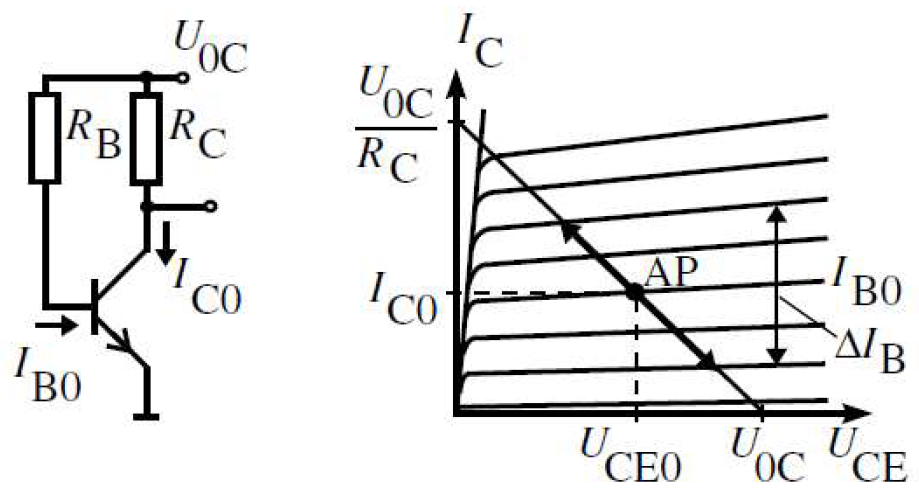
\includegraphics[width=1\textwidth]{images/emitterStufe.png}

Die Speisung VDD(U0C) sei 5V

\begin{enumerate}
\item Wie gross wird der Kollektorstrom IC0 im Arbeitspunkt, wenn die Arbeitspunkt-Spannung
UCE0=VDD/2 betragen soll?
\item Wie gross wird der Basisstrom IB0 für den Arbeitspunkt, wenn Sie einen npn-Transistor zur Verfügung haben und dieser genau den mittleren Stromverstärkungsfaktor hFE aufweist?
\item Wie gross wird die zu erwartende Basis-Emitter-Spannung VBE0 bei Ihrem Arbeitspunkt?
\end{enumerate}

\newpage
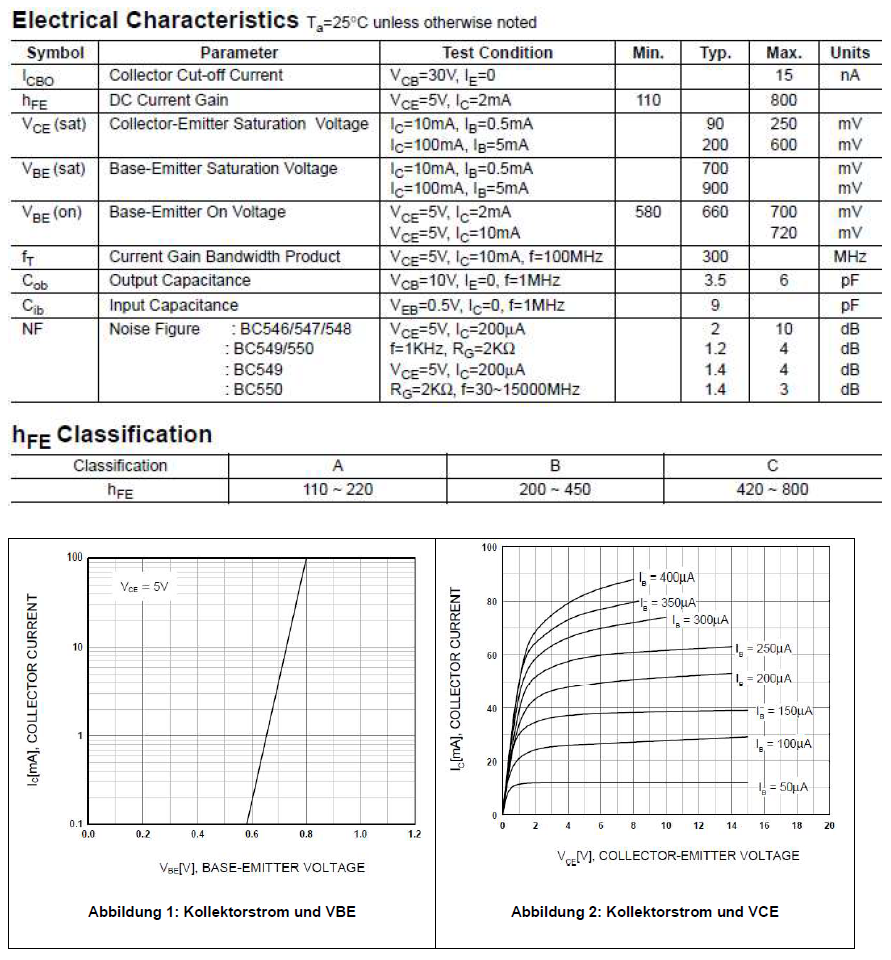
\includegraphics[width=1.2\textwidth]{images/datasheetBC547.png}